\part{Progettare la CPU}

\chapter{Elaborare un'istruzione}
Le fasi di esecuzione di un'istruzione sono:
\begin{itemize}
    \item \textbf{caricamento} di una istruzione dalla memoria alla CU;
    \item \textbf{decodifica} della istruzione e lettura argomenti dai registri;
    \item \textbf{esecuzione} (attivazione delle unità funzionali necessarie);
    \item \textbf{accesso} alla memoria;
    \item \textbf{scrittura} dei risultati nei registri;
    \item \textbf{aggiornamento} del PC (normale/salti condizionati/salti non condizionati).
\end{itemize}

Le istruzioni che la CPU può eseguire sono: accesso alla memoria: \verb|lw, sw| (di tipo I); salti condizionati: \verb|beq| (di tipo I); operazioni aritmetico-logiche: \verb|add, sub, sll, slt ,...| (di tipo R); salti non condizionati \verb|j, jal| (di tipo J); operazioni con costanti \verb|li, addi, subi, ...| (di tipo I). 

Ricordiamo il formato delle tre istruzioni MIPS (r, i, j type) codificate nella memoria:
\begin{figure}[H]
    \centering
    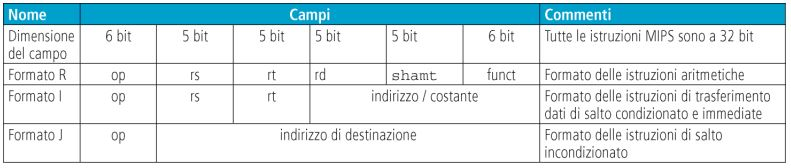
\includegraphics[width=14cm]{Capitoli/CPU/imgCpu/istruzioniMips.JPG}
\end{figure}


\chapter{Unità della CPU}

\section{Memoria delle istruzioni, PC, adder}
\begin{wrapfigure}{r}{0.5\textwidth}
    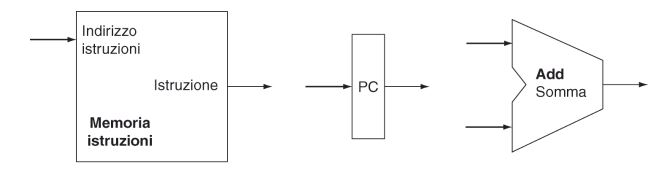
\includegraphics[width=8cm]{Capitoli/CPU/imgCpu/memoriaPcAdder.JPG}
\end{wrapfigure}
La \textit{memoria istruzioni} riceve in input un indirizzo da 32 bit e restituisce in output l'istruzione (opcode) situata nell'indirizzo di input.

Il \textit{program counter} o PC è un registro che contiene l'indirizzo dell'istruzione corrente. 

Tramite l'\textit{adder}, se necessario, si calcolerà la nuova destinazione del program counter, per leggere una successiva istruzione o per un salto relativo.


\section{Registri e ALU}
Il \textit{blocco dei registri} contiene 32 registri a 32 bit, indirizzabili tramite 5 bit ($2^5=32$). E' formato da 3 porte da 5 bit per indicare quali registri leggere (\verb|rs, rt|) e in quale scrivere (\verb|rd|), 3 porte dati (a 32 bit), di cui una in ingresso per il valore da memorizzare e 2 di uscita per i valori letti (capiremo dopo il perchè di questa doppia scelta) e il segnale \verb|RegWrite| che abilita (se 1) la scrittura nel registro di scrittura.

L'\textit{ALU}, invece, riceve due valori interi a 32 bit e svolge l'operazione indicata dal segnale \verb|Op.ALU|. Oltre al risultato da 32 bit produce un segnale \verb|Zero| riportato se il risultato è zero.

\begin{figure}[H]
    \centering
    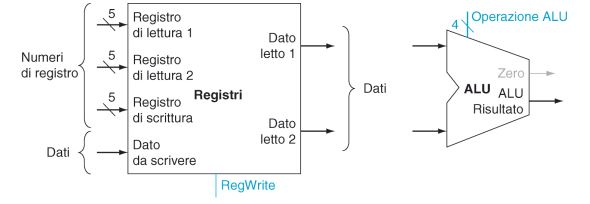
\includegraphics[width=10cm]{Capitoli/CPU/imgCpu/registriAlu.JPG}
\end{figure}

Notiamo che i bit dell'\verb|Op.ALU|, dagli originali 6, si riducono a 4. Ciò avviene perchè è stato stabilito che bastano solamente 4 bit per rappresentare le operazioni che l'ALU può svolgere.

\begin{figure}[H]
    \centering
    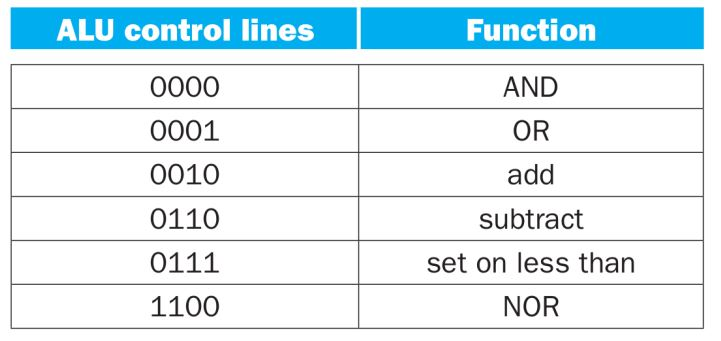
\includegraphics[width=8cm]{Capitoli/CPU/imgCpu/opAlu.JPG}
    \caption{Operazioni dell'ALU}
\end{figure}

\section{Memoria dati ed unità di estensione del segno}
L'\textit{unità di memoria} viene utilizzata per tutte quelle operazioni che richiedono accessi alla memoria come \verb|lw, sw|.
L'unità di memoria riceve un indirizzo (da 32 bit) che indica quale word della memoria va letta/scritta, riceve il segnale \verb|MemRead| che abilita la lettura dall’indirizzo (se \verb|lw|), riceve un dato da 32 bit da scrivere in memoria a quell’indirizzo (se \verb|sw|), riceve il segnale di controllo \verb|MemWrite| che abilita (1) la scrittura del dato all’indirizzo.

L’\textit{unità di estensione del segno} è di grande aiuto per quelle istruzioni che utilizzano 16 bit ma per l'operazione se ne richiedono 32. Nello specifico serve a trasformare un intero relativo (in CA2) da 16 a 32 bit.
\begin{figure}[H]
    \centering
    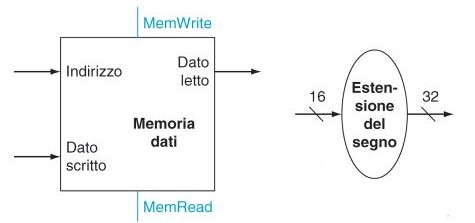
\includegraphics[width=10cm]{Capitoli/CPU/imgCpu/memoriaDatiEEstensioneSegno.JPG}
\end{figure}

\section{Fetch della istruzione/aggiornamento del PC}
L'\textit{aggiornamento del program counter} viene effettuato tramite un adder seguendo vari passaggi. Nel PC si trova l'indirizzo dell'istruzione, l'istruzione viene letta, mentre avviene la lettura il PC viene incrementato di 4 bit (1 word) e il valore viene inserito nuovamente nel PC.
\begin{figure}[H]
    \centering
    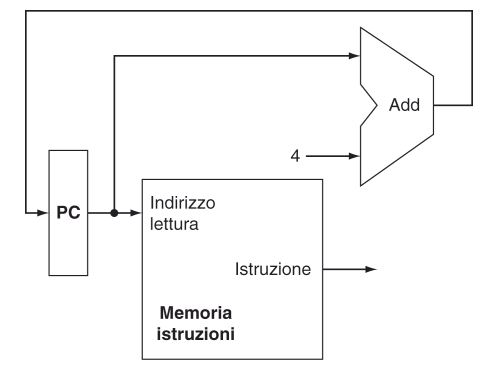
\includegraphics[width=6cm]{Capitoli/CPU/imgCpu/fetchPc.JPG}
\end{figure}

\begin{example*}
    Proviamo a rappresentare il percorso delle seguenti istruzioni con i moduli visti fin ora: 
    
    \verb|add $s0, $s1, $s2; lw $s0, 4($s1); sw $s0, 4($s1); beq s0, $s1, 0x00000014|.
    Ricordiamo che per prendere delle scelte utilizziamo i multiplexer. In particolare a seconda del segnale di controllo \verb|ALUSrc| viene selezionata la porta corrispondente del MUX di sinistra. Per calcolare l’indirizzo di accesso alla memoria si usa la stessa ALU. Il risultato dell’ALU o della lw viene selezionato da \verb|MemtoReg| che comanda il MUX a destra.
\begin{figure}[H]
    \centering
    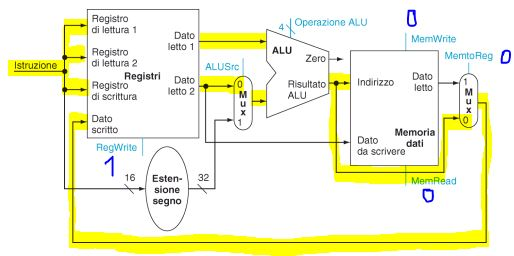
\includegraphics[width=8cm]{Capitoli/CPU/imgCpu/esAdd.JPG}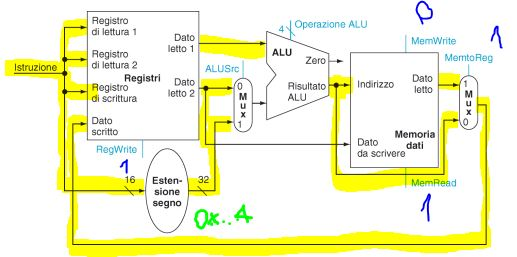
\includegraphics[width=8cm]{Capitoli/CPU/imgCpu/esLw.JPG}
    \caption{add \$s0, \$s1 \$s2 e lw \$s0, 4(\$s1)}
\end{figure}
\begin{figure}[H]
    \centering
    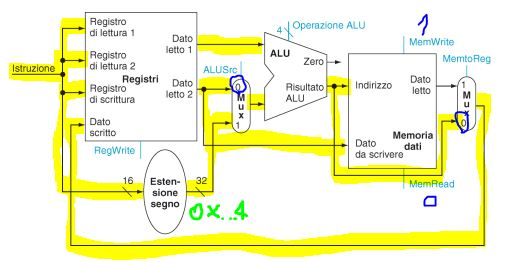
\includegraphics[width=8cm]{Capitoli/CPU/imgCpu/esSw.JPG}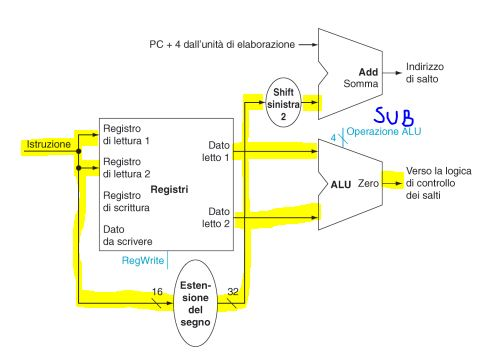
\includegraphics[width=8cm]{Capitoli/CPU/imgCpu/esBeq.JPG}
    \caption{sw \$s0, 4(\$s1) e beq s0, \$s1, 0x00000014}
\end{figure}
\end{example*}

\section*{CPU (quasi) completa}
Con l'unione di tutti i moduli visti precedentemente, con l'aggiunta dei multiplexer come branch di scelte, Control Unit (il cervello della CPU che comanda le scelte da prendere) e la logica del salto (incrementa il program counter), otteniamo il seguente schema della CPU:
\begin{figure}[H]
    \centering
    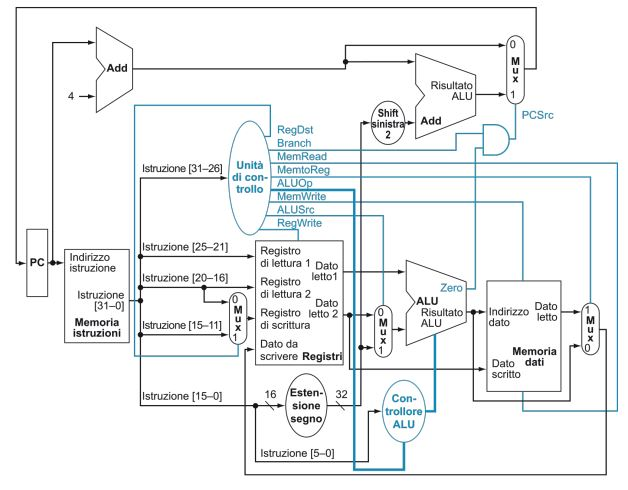
\includegraphics[width=15cm]{Capitoli/CPU/imgCpu/CpuCompleta.JPG}
    \caption{Schema della CPU}
\end{figure}

\section{Aggiungere i Jump}
Supponiamo di voler aggiungere la nuova istruzione, J (\textit{Jump}). Ricordiamo la codifica dei salti (formato J):
\begin{table}[H]
    \centering
    \begin{tabular}{|c|c|}
         \hline \hspace{.5cm}000010\hspace{.5cm} & \hspace{2cm}indirizzo\hspace{2cm}\phantom{}\\\hline
    \end{tabular}
    \begin{tabular}{cc}
         \hspace{.1cm}31-26\hspace{.8cm} & \hspace{2.2cm}25:0\hspace{2cm}\phantom{}\\
    \end{tabular}
\end{table}

L'indirizzo di destinazione del salto è contenuto nei 26 bit (25:0), ed è un indirizzo assoluto, ovvero non relativo al PC come ad esempio per i brach. Per tanto questo indirizzo va moltiplicato per 4 perché le istruzioni sono allineate, così da ricavare un'istruzione di 28 bit. E i mancanti 4 bit (per ottenere un totale di 32 bit) verranno presi dal PC+4.

Nello specifico le operazioni da svolgere saranno le seguenti:
\begin{equation*}
    \text{PC} \Longleftarrow (\text{\textbf{shift left} di 2 bit di Istruzione}[25-0]) \text{ \textbf{OR} } (\text{PC}+4)[31-28]
\end{equation*}

Allo schema della CPU non resta che aggiungere lo shift left di 2 bit con input a 26 bit e MUX per selezionare il nuovo PC (l'OR dei 28 bit ottenuti con i 4 del PC+4 si ottiene dalle connessioni). E' importante ricordarsi di settare i controlli \verb|RegWrite| e \verb|MemWrite| a 0 per evitare modifiche a registri e alla memoria. [\textit{\textcolor{cyan}{Vedi Figura \ref{fig:jumpCpu}}}]\\

L'istruzione Jal (\textit{Jump And Link}) è sempre codificata come tipo J, inoltre le operazioni preliminari sono le stesse del Jump con l'aggiunta del comando \verb|$ra <- PC+4|. 

Le unità funzionali previste saranno le stesse di quelle utilizzate per il Jump, con l'aggiunta di un MUX per selezionare il valore di PC+4 come valore di destinazione e un MUX per selezionare il numero del registro \$ra come destinazione. Infatti il primo di questi MUX conterrà il PC+4, mentre il secondo il valore 31 che rappresenta il $31^o$ registro del MIPS che è esattamente il registro \$ra. La CU infine deve produrre un segnale \verb|Link| per attivare i due nuovi MUX. [\textit{\textcolor{red}{Vedi Figura \ref{fig:jumpCpu}}}]\\

L'istruzione Jr (\textit{Jump to Register}) è di tipo R, ricordiamo che questa operazione permette di trasferire nel PC il contenuto del registro specificato. Per tanto oltre alle unità già previste per i jump precedenti non resta che aggiungere un MUX per selezionare il PC dall'uscita del blocco registri. L'unico segnale necessario è il \verb|JumpToReg| che abilita il MUX per inserire in PC il valore del registro. [\textit{\textcolor{yellow}{Vedi Figura \ref{fig:jumpCpu}}}]

\begin{figure}[ht]
    \centering
    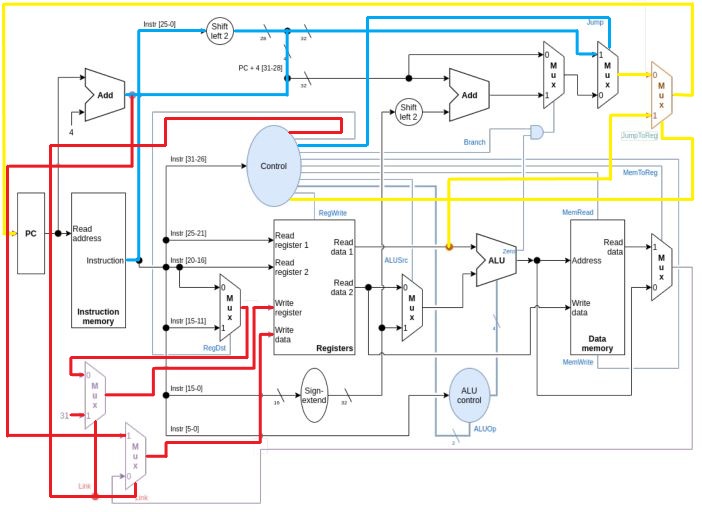
\includegraphics[width=14cm]{Capitoli/CPU/imgCpu/jumpCpuMod.png}
    \caption{Aggiunta dei Jump}
    \label{fig:jumpCpu}
\end{figure}

\section{Segnali di controllo}
A questo punto un'interessante esercizio potrebbe essere quello di individuare il valore di tutti i segnali di controllo della CPU delle operazioni: \verb|tipo R|, \verb|lw|, \verb|sw|, \verb||beq, \verb|j|.
\begin{figure}[H]
    \centering
    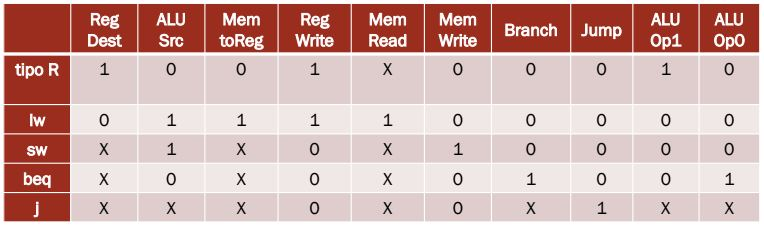
\includegraphics[width = 12cm]{Capitoli/CPU/imgCpu/segnaliDiControlloCpu.JPG}
    \caption{Segnali di controllo delle principali operazioni}
    \label{fig:segnaliDiControllo}
\end{figure}
\phantom{}\\
Può accadere che durante l'esecuzione di un'istruzione ci accorgiamo che la CPU genera segnali errati. I passi da seguire quando si verifica un \textit{malfunzionamento della CPU} sono: individuare quale combinazione di segnali viene generata ed individuare quali istruzioni vengono influenzate dalle nuove combinazioni.
Una volta individuate le nuove funzionalità (fallaci) delle istruzioni possiamo cercare di scrivere un breve programma che evidenzia se la CPU sia mal funzionante o meno.

\chapter{Pipeline}
Nel capitolo precedente abbiamo analizzato il processo di elaborazione di un'istruzione. Per semplicità possiamo riassumere le varie fasi dell'istruzione in:
\begin{itemize}
    \item \textbf{Fetch}: carica l’istruzione dalla memoria;
    \item \textbf{Instruction Decode}: la CU decodifica l’istruzione e vengono letti gli argomenti dai registri;
    \item \textbf{Execution}: l’ALU fa il calcolo necessario (tipo R o accesso alla memoria o branch);
    \item \textbf{Memory access}: viene letta/scritta la memoria (lw e sw);
    \item \textbf{Write Back}: il risultato dell’ALU o quello letto dalla memoria viene messo nel registro dest.
\end{itemize}

Notiamo come eseguendo un'istruzione per volta, la CPU è per l’80\% inutilizzata. Da qui nasce l'idea di utilizzare le \textit{pipeline} ovvero dei processi per incrementare il throughput, ovvero la quantità di istruzioni eseguite in una data quantità di tempo, parallelizzando i flussi di elaborazione di più istruzioni. In altre parole vogliamo ottimizzare i processi della CPU rendendo ogni unità funzionale autonoma di passare all'istruzione successiva. In questo modo possono essere eseguite fino a cinque istruzioni contemporaneamente nel caso migliore (anche se noteremo che non sempre sarà possibile).

\begin{figure}[H]
    \centering
    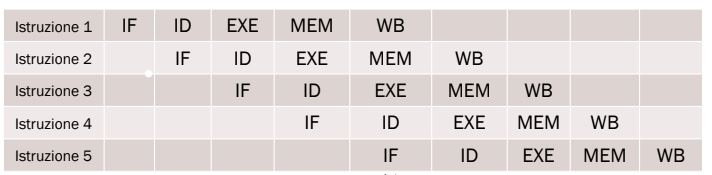
\includegraphics[width = 12cm]{Capitoli/CPU/imgCpu/pipeline_es.JPG}
    \caption{Cinque istruzioni ottimizzate con le pipeline}
    \label{fig:pipline_es}
\end{figure}

Ad ogni colpo di clock una istruzione viene completata dalla pipeline. Possiamo arrivare a quintuplicare (idealmente) il throughput.

\begin{example*}
    Analizziamo i risultati delle seguenti istruzioni \verb|lw $1,100($0)| \verb|lw $2,200($0)| \verb|lw $3,300($0)|.
    
    Con un approccio sequenziale delle istruzioni otterremmo il seguente risultato:
    \begin{figure}[H]
        \centering
        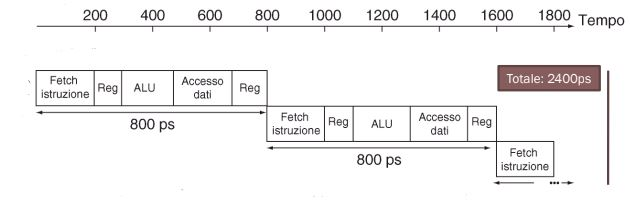
\includegraphics[width = 12cm]{Capitoli/CPU/imgCpu/pipeline_es_lw.JPG}
    \end{figure}
    
    Mentre con le pipeline:
    \begin{figure}[H]
        \centering
        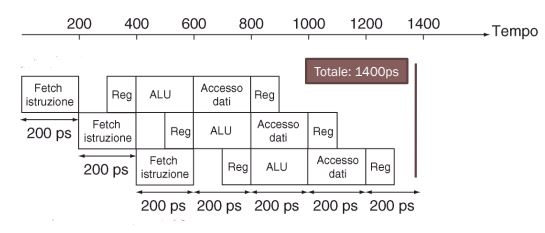
\includegraphics[width = 12cm]{Capitoli/CPU/imgCpu/pipeline_es_lw1.JPG}
    \end{figure}
    
    Ogni componente lavora in maniera autonoma, senza aspettare il risultato dell'istruzione precendente (non sempre è possibile), in modo da passare all'istruzione successiva e migliorare i tempi di elaborazione.
\end{example*}

E' possibile utilizzare in maniera efficiente le pipeline nell'architettura MIPS perchè di tipo RISC (vedi \ref{architettureCISCeRISC}) infatti, con questo tipo di struttura, si presentano numerosi vantaggi come: i registri sorgente sono nella stessa posizione, la lettura di \verb|rs| viene fatta durante la fase ID, gli operandi in memoria solo utilizzati solo per \verb|lw| e \verb|sw|, il trasferimento del risultato avviene sempre in coda, è necessario un singolo accesso in memoria per dato.

\section{Criticità (Hazard)}
Ovviamente non è sempre possibile sfruttare questi vantaggi in maniera efficiente. Si possono presentare dei casi in cui:
\begin{itemize}
    \item le risorse hardware non sono sufficienti (\textit{structural hazard});
    \item il dato necessario non è ancora pronto (\textit{data hazard});
    \item la presenza di un salto cambia il flusso di esecuzione delle istruzioni (\textit{control hazard}).
\end{itemize}

\begin{example*}
    Le criticità più frequenti sono quelle legate ai dati. Ad esempio \verb|add $s0,$t0,$t1| \verb|sub $t2,$s0,$t3|.
    \begin{figure}[H]
        \centering
        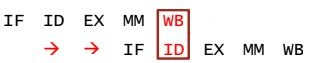
\includegraphics[width = 8cm]{Capitoli/CPU/imgCpu/hazard_es.JPG}
    \end{figure}
    
    Non può essere eseguita la lettura degli elementi della seconda istruzione finchè non si esegue il write back. Inoltre si possono inserire in parallelo il WB e l'ID perchè a livello di architettura viene eseguito prima il write e dopo il read (proprio per risparimiare tempo in questo tipo di casi).
\end{example*}

\section{Propagazione (Forwarding)}
In alcuni casi l’informazione necessaria è già presente nella pipeline, prima del WB. Possiamo, in questi casi inserire nel datapath delle "scorciatoie" che recapitano il dato all’unità funzionale che ne ha bisogno senza aspettare la fase di WB.

E' possibile utilizzare la propagazione solo quando lo stadio che deve ricevere il dato è successivo a quello che lo produce nel diagramma temporale della pipeline.

Riprendendo l'esercizio precedente possiamo creare un collegamento tra EX e ID per lavorare direttamente sul dato interessato:
\begin{figure}[H]
    \centering
    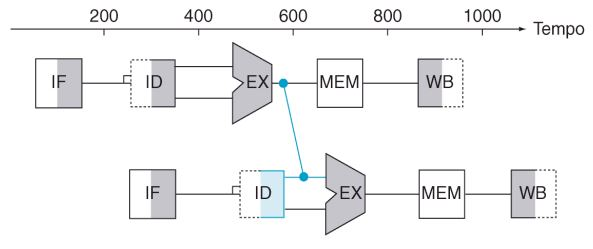
\includegraphics[width = 10cm]{Capitoli/CPU/imgCpu/propagazione_es.JPG}
\end{figure}

\section{Bolla (bubble)}
Se la fase che ha bisogno del dato si trova prima (nel tempo) di quella che lo produce sarà necessario inserire una attesa (stallo o bolla). Una bolla è un'istruzione che non fa niente e deve essere inserita perchè la CPU non può produrla o aspettare lo stallo. Anche se è possibile utilizzare una bolla è sempre meglio inserire altre istruzioni successive per guadagnare in termini di efficienza.

\begin{example*}
    Con le istruzioni \verb|lw $s0,20($t1)| \verb|sub $t2,$s0,$t3| siamo obbligati ad utilizzare una bolla perchè per la seconda istruzione ci serve il valore memorizzato nella prima:
\begin{figure}[H]
    \centering
    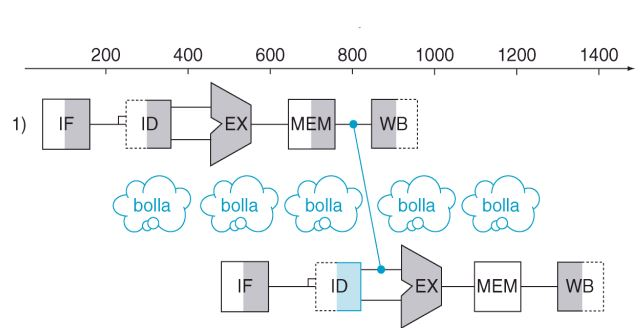
\includegraphics[width = 10cm]{Capitoli/CPU/imgCpu/bolla.JPG}
\end{figure}
\end{example*}

\section{Hazard sul controllo}
Quando abbiamo a che fare con istruzioni di controllo, l’istruzione successiva può essere caricata solo dopo che il salto è stato deciso. Sono inoltre necessari 2 stalli se la \verb|beq| viene decisa in EXE o 1 se viene decisa in ID.

\begin{example*}
    Consideriamo queste tre istruzioni \verb|add $4,$5,$6| \verb|beq $1,$240| \verb|or $7,$8,$9|:
    \begin{figure}[H]
        \centering
        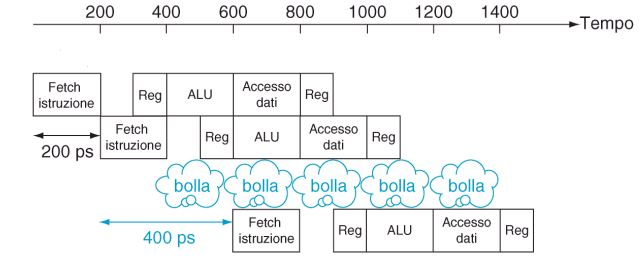
\includegraphics[width=12cm]{Capitoli/CPU/imgCpu/hazard_controllo.JPG}
    \end{figure}
\end{example*}

Per diminuire i control hazard possiamo:
\begin{itemize}
    \item \textit{Anticipare la decisione}: se la \verb|beq| viene calcolata nell'ALU, nella fase EXE ci saranno 2 istruzioni da "buttare", se invece la \verb|beq| viene decisa nella fase ID è sufficiente "buttare" 1 istruzione;
    \item \textit{Ritardare il salto}: se l’istruzione che segue la \verb|beq| viene sempre eseguita anche se viene effettuato il salto, si elimina lo stallo;
    \item \textit{Branch prediction}: la CPU osserva i salti eseguiti e cerca di pre-caricare l’istruzione (seguente o di destinazione) eseguita più spesso.
\end{itemize}

\section{Registri di pipeline}
Riprendiamo ciò che abbiamo visto precedentemente con questa semplice immagine:
\begin{figure}[H]
    \centering
    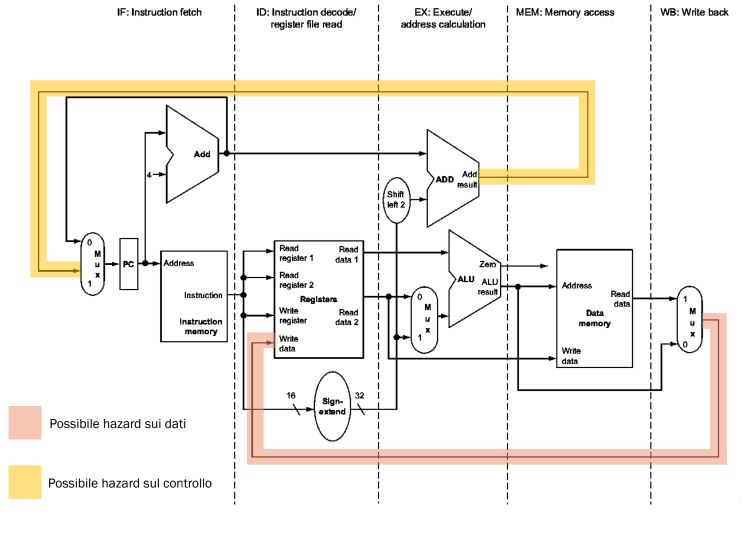
\includegraphics[width = 14cm]{Capitoli/CPU/imgCpu/cinque_fasi.JPG}
    \caption{Unità funzionali nelle cinque fasi}
    \label{fig:cinque_fasi}
\end{figure}

In molti casi si è presentata la necessità di utilizzare i valori contenuti nelle fasi precedenti per svolgere correttamente più istruzioni alla volta. In tal senso vengono in nostro aiuto i \textit{registri di pipeline} che ci permettono di salvare, in registri di appoggio, il contenuto dopo ogni fine fase. 

I registri di pipeline sono in totale quattro, perchè sull'ultima unità funzionale (\verb|Write Back|) non servono valori da memorizzare in quanto questi verranno direttamente scritti nel registro destinazione. Inoltre questi registri hanno dimensioni diverse tra di loro in base alla quantità di informazioni che devono memorizzare all'uscita dell'unità funzionale.

\begin{figure}
    \centering
    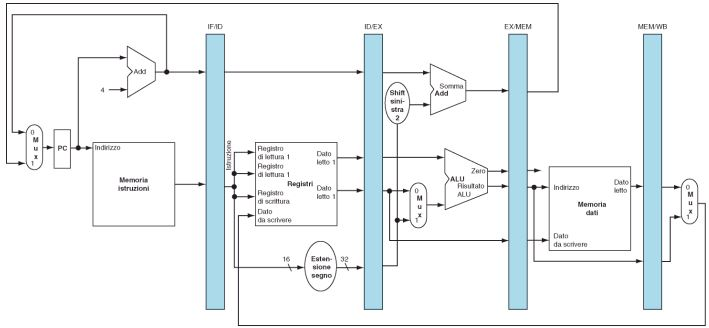
\includegraphics[width = 12cm]{Capitoli/CPU/imgCpu/registri_di_pipeline.JPG}
    \caption{Registri di pipeline}
    \label{fig:registri_di_pipeline}
\end{figure}

Per evitare di sovrascrivere i registri delle unità funzionali durante l'esecuzione in pipeline di altre istruzioni, dobbiamo salvare il valore del registro di destinazione e propagare i segnali di controllo. Possiamo dividere i segnali di controllo delle fasi esecutive in tre gruppi: fase EXE, fase MEM, fase WB:

\begin{figure}[H]
    \centering
    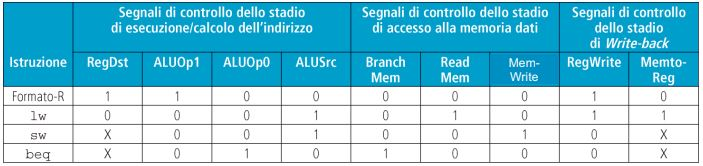
\includegraphics[width = 12cm]{Capitoli/CPU/imgCpu/segnali_pipeline.JPG}
    \caption{Segnali di controllo delle pipeline}
    \label{fig:segnali_pipeline}
\end{figure}

Questi segnali devono essere passati di fase in fase nei registri della pipeline. Cosicchè ad ogni fase salviamo i dati (letti dai registri o dalla parte immediata) ed i segnali di controllo della stessa istruzione (generati dalla CU):

\begin{figure}[H]
    \centering
    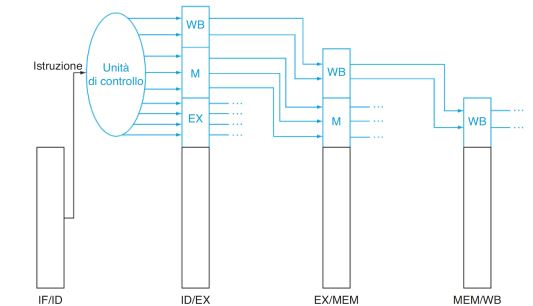
\includegraphics[width = 12cm]{Capitoli/CPU/imgCpu/propagazione_segnali_pipeline.JPG}
    \caption{Propagazione dei segnali di controllo in pipeline}
    \label{fig:propagazione_segnali_pipeline}
\end{figure}

Ora possiamo finalmente dare uno sguardo allo schema della CPU con l'aggiunta delle pipeline, anche se nei prossimi paragrafi verrà leggermente aggiornato:

\begin{figure}[H]
    \centering
    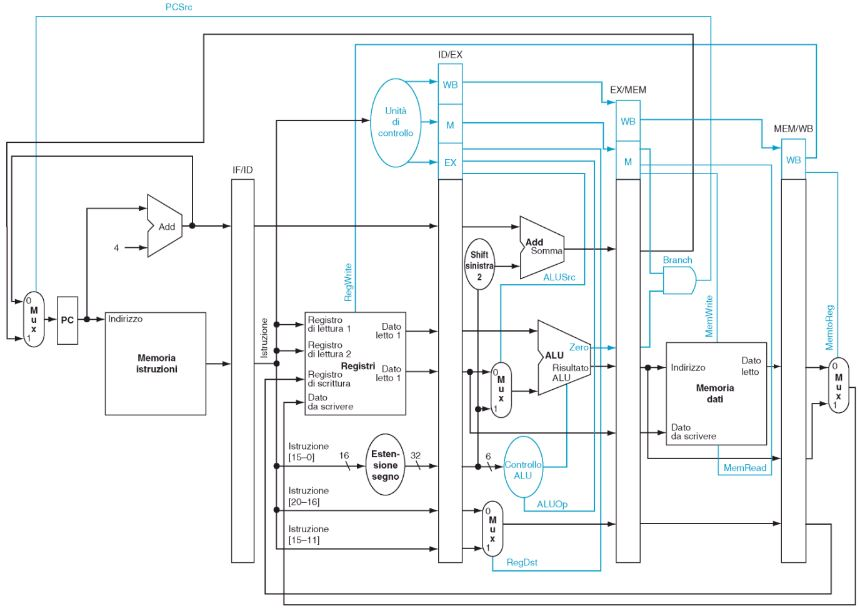
\includegraphics[width = 14cm]{Capitoli/CPU/imgCpu/cpu_con_pipeline.JPG}
    \caption{CPU con pipeline}
    \label{fig:cpu_con_pipeline}
\end{figure}

\section{Realizzare il forwarding}
Torniamo a parlare di forwarding, e in pariticolar modo di quello in EXE, ovvero quel processo che ci permette di sostituire il valore letto dal blocco registri con quello prodotto dall'istruzione precedente.

Con la struttura della CPU vista finora, per realizzare il forwarding, vogliamo apportare delle modifiche al datapath, ovvero iniserire un MUX prima dell'ALU per distinguere tre casi:
\begin{enumerate}
    \item \textit{Non c'è forwarding}: il valore per la ALU viene dal registro ID/EX della pipeline;
    \item \textit{Forwarding dall'istruzione precedente}: il valore per la ALU viene dal registro EX/MEM della fase precedente;
    \item \textit{Forwarding dalla seconda istruzione precedente}: il valore per la ALU viene dal registro MEM/WB della fase precedente.
\end{enumerate}

Quindi per realizzare il forwarding dobbiamo inserire due MUX prima dell'ALU (uno per il registro \verb|rs| e uno per \verb|rt|) e creare dei segnali per il forwarding:
\begin{figure}[H]
    \centering
    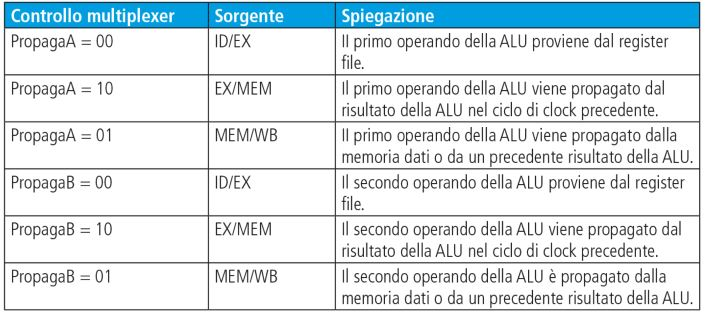
\includegraphics[width = 12cm]{Capitoli/CPU/imgCpu/segnali_forwarding.JPG}
    \caption{Segnali per il forwarding}
    \label{fig:segnali_forwarding}
\end{figure}

\begin{nota*}
    E' possibile realizzare il forwarding anche nella fase ID (necessario SOLO se la \verb|beq| viene anticipata in ID) e nella fase MEM (necessario SOLO se \verb|lw $rt|, ... è subito seguita da \verb|sw $rt|, ...).
\end{nota*}

\begin{figure}[H]
    \centering
    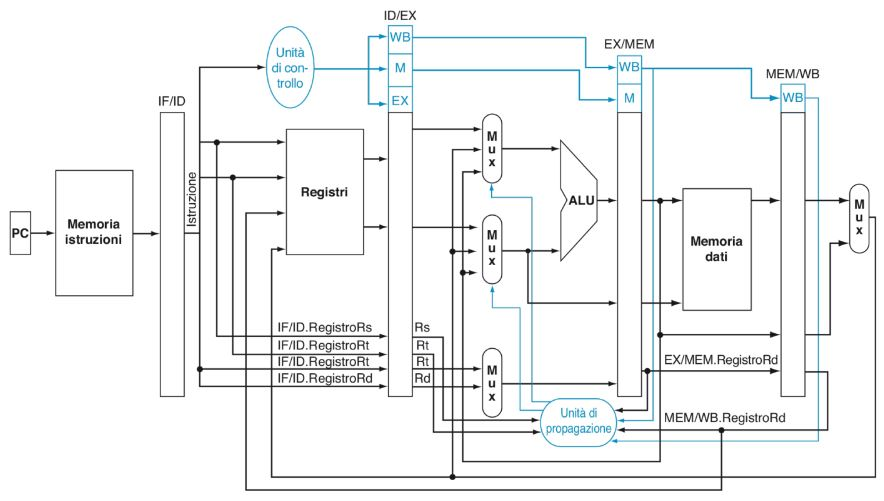
\includegraphics[width = 14cm]{Capitoli/CPU/imgCpu/cpu_con_forwarding.JPG}
    \caption{CPU con forwarding}
    \label{fig:cpu_con_forwarding}
\end{figure}

\section{Realizzare lo stallo}
Come abbiamo visto in precedenza talvolta l’istruzione deve attendere che sia pronto il dato perché possa avvenire il forwarding.

Per fermare l’istruzione con uno stallo, dobbiamo (nella fase ID) annullare l’istruzione che deve attendere (bolla), azzerarando i segnali di controllo \verb|MemWrite| e \verb|RegWrite| nonché \verb|IF/ID.Istruzione| e rileggere la stessa istruzione affinché possa essere rieseguita un ciclo di clock dopo impedendo quindi che il PC si aggiorni.

\begin{figure}[H]
    \centering
    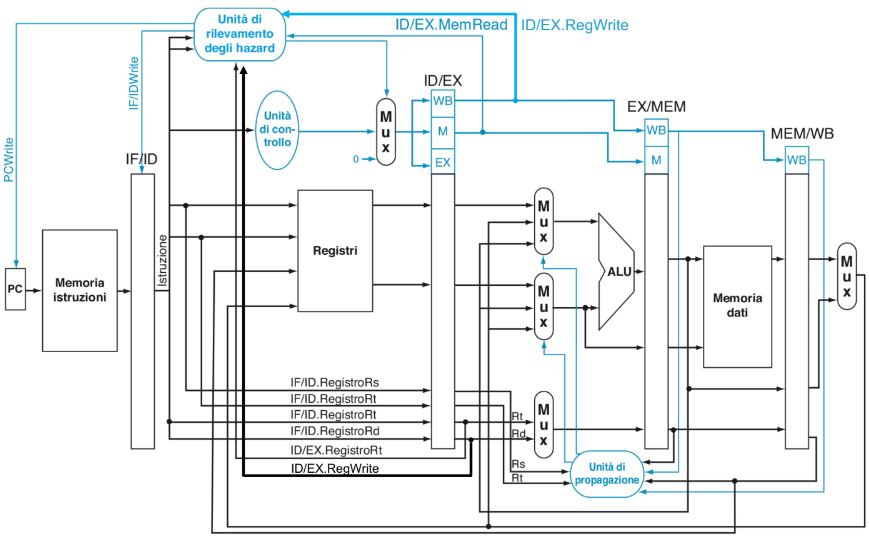
\includegraphics[width = 14cm]{Capitoli/CPU/imgCpu/cpu_con_stallo.JPG}
    \caption{CPU con stallo}
    \label{fig:cpu_con_stallo}
\end{figure}


\section{Anticipare i salti}
Per quanto visto finora ogni istruzione viene riconosciuta nella fase ID mentre un’altra viene caricata, quindi il \verb|Jump| implica almeno uno stallo per l’istruzione successiva. Inoltre, quando deve essere eseguito un salto, la pipeline è mezza piena e le istruzioni seguenti già caricate vanno eliminate dalla pipeline. Per eliminare l’istruzione con uno stallo, occorre (nella fase ID), annullare l’istruzione inutile (bolla), ovvero azzerare i segnali di controllo \verb|MemWrite| e \verb|RegWrite| e IF/ID, e aggiornare il PC affinché possa leggere la destinazione al prossimo colpo di clock.

Per saltare con la J in fase IF occorre: anticipare il riconoscimento della istruzione (che normalmente fa la CU in fase ID) comparando col valore dell'\verb|OpCode| della J (000010); spostare la logica di aggiornamento del PC alla fase IF effettuando uno shift logico a 2 dei 26 bit meno significativi dell'istruzione e aggiungendo 4 bit più significativi di PC+4. Il risultato è una \verb|Jump| anticipata che non introduce più stalli.

L’istruzione \verb|beq| normalmente usa la ALU per fare il confronto, per cui: il salto avviene normalmente dopo la fase EXE (nella fase MEM); in caso di salto, le 2 istruzioni seguenti (già caricate) vanno annullate. Per anticipare la decisione di salto alla fase ID occorre non usare la ALU ma inserire un comparatore tra i due argomenti letti dal blocco registri, spostando la logica di salto ed il calcolo del salto relativo dalla fase EXE alla fase ID.

\section{Predire i salti}
Molte volte il responsabile di cali di efficienza è il tipo di codice che viene usato dalla \verb|beq|, soprattutto nei cicli: se il test è all'inizio, seguito dal corpo del ciclo, la \verb|beq| fa un solo salto alla fine del ciclo; se il test è alla fine, dopo il corpo, la \verb|beq| effettua molti salti e in un solo caso continuerà.

La CPU vista finora presume che il salto non venga effettuato (branch not taken), se si potesse "prevedere" il salto si potrebbero caricare le istruzioni giuste ed evitare stalli.

Ad ogni istruzione di salto possiamo associare bit che contano i salti già effettuati per decidere se sia più probabile che il salto venga effettuato o meno. Con un bit si può rappresentare l’informazione l’ultima volta il salto è stato effettuato, ma nel realizzare un ciclo la previsione sarà sbagliata 2 volte: entrando e uscendo. Con due bit, invece, si può realizzare una macchina a stati finiti che necessita di due errori consecutivi per cambiare previsione, quindi incorre in meno errori nei cicli.

\begin{figure}[H]
    \centering
    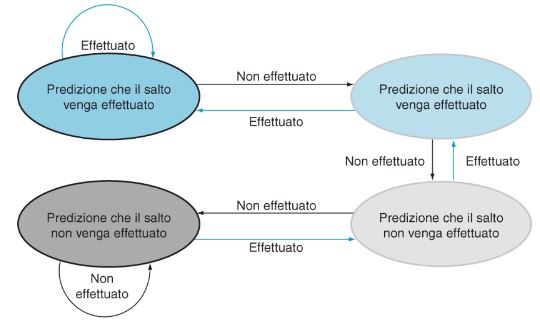
\includegraphics[width = 10cm]{Capitoli/CPU/imgCpu/predizione_salti.JPG}
    \caption{Macchina a stati finiti per la predizione dei salti}
    \label{fig:predizione_salti}
\end{figure}


\chapter{Cache}

Fare tanti accessi alla memoria risulta essere un'operazione dispendiosa in termini di tempo (la RAM è circa 10-100 volte più lenta del processore) o di costi (una memoria tanto è veloce quanto costosa), per tanto vogliamo sviluppare un nuovo modello di memoria che ci aiuta in queste operazioni. 

Quando utilizziamo la memoria non abbiamo bisogno di tutte le informazioni in essa contenute. Al pari della memoria umana, vorremmo dare priorità ai dati che vengono letti con maggiore frequenza e, di conseguenza, meno priorità a quelli che vengono letti di meno.
Questa è l'idea alla base della \textit{cache}, una memoria prioritaria, che si basa sul principio di località temporale: «un programma tende ad accedere allo stesso elemento in momenti vicini tra loro».

Possiamo vedere la cache come una memoria ridotta formata da N linee.
Quando la CPU richiede un indirizzo, se il blocco corrispondente è presente nella cache allora il dato è caricato (\textit{HIT}), altrimenti il dato è preso dalla RAM e il blocco è copiato nella cache (\textit{MISS}).

Le N linee della cache contengono: 1 \textit{bit di validità} che indica se la linea contiene dati validi, il campo \textit{tag} che distingue quale blocco della memoria è nella linea evitando eventuali collisioni e il \textit{blocco} memorizzato nella linea.
\begin{figure}[H]
    \centering
    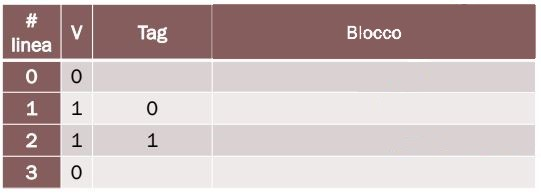
\includegraphics[width = 10cm]{Capitoli/CPU/imgCpu/cache_schema.JPG}
    \caption{Schema della cache}
    \label{fig:schema_cache}
\end{figure}

\section{Direct mapping}
Per guadagnare di efficienza la cache deve essere indipendente dal processore, per tanto le informazioni vengono memorizzate tramite il \textit{direct mapping}. In questo modo non si deve interrogare la CPU ma basta semplicemente leggere l'indirizzo dell'istruzione per ottenere l'\textit{offset}, l'\textit{indice di linea} e il \textit{tag}.
\begin{figure}[H]
    \centering
    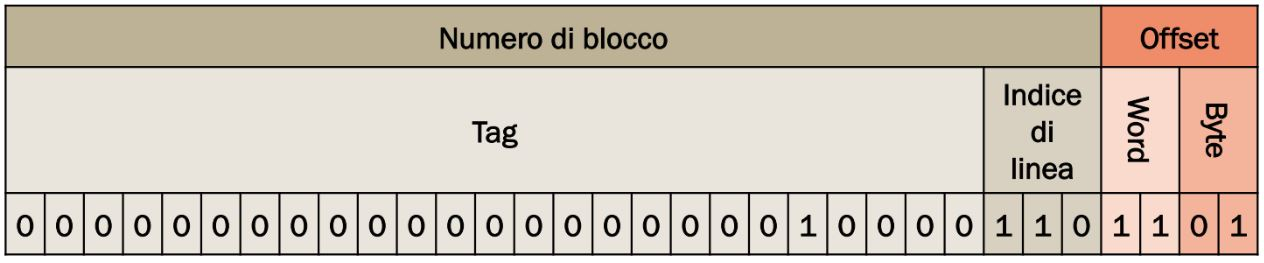
\includegraphics[width = 14cm]{Capitoli/CPU/imgCpu/direct_mapping.JPG}
    \caption{Direct mapping}
    \label{fig:direct_mapping}
\end{figure}
Il blocco letto si posizionerà nella linea della cache ottenuta dal numero di blocco \% (modulo) il numero di linee disponibili nella cache.

\begin{example*}
    Supponiamo di avere una cache che contiene 8 linee di cui ogni blocco può contenere 4 word = 16 byte,  e l'indirizzo $2157 = 0x0000 086D$. Il numero di blocco si ottiene $2157 / 16 = 134 = 0x86$, a sua volta il numero di blocco si divide in tag e indice di linea: tag = $134 / 8 = 16 = 0x10$; Indice di linea = $134 \% 8 = 6 = 0x6$. Per l'offset infine calcoliamo $2157 \% 16 = 13 = 0xD$.
\end{example*}
\begin{figure}
        \centering
        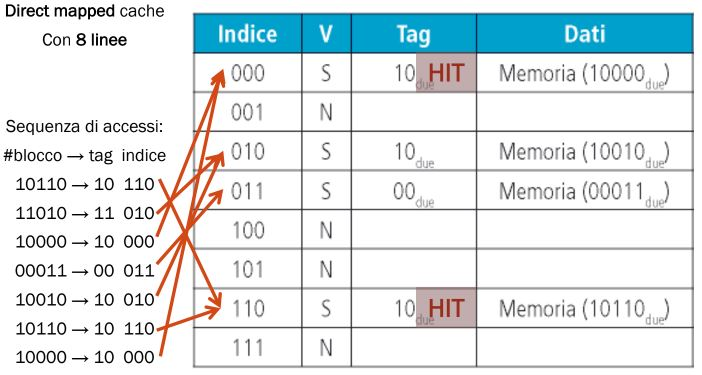
\includegraphics[width = 12cm]{Capitoli/CPU/imgCpu/es_direct_mapping.JPG}
        \caption{Esempio di direct mapping}
        \label{fig:es_direct_mapping}
    \end{figure}
    
\section{Determinare HIT/MISS}
Supponiamo di avere una cache di 256 linee con blocchi da 16 word. Il procedimento per determinare se il processore trova che la posizione di memoria è in cache (\textit{HIT}) o non è in memoria (\textit{MISS}) è riassunto in Figura \ref{fig:hit_miss}. 
Notiamo come in caso di HIT, si va all'indice di linea corrispondente, si verifica se il tag è uguale a quello del blocco e in tal caso il processore può leggere la parola direttamente dalla cache. In caso di MISS, invece, tramite un MUX, si prende dato relativo all'offset del blocco e si crea una nuova entità, che comprende l'etichetta appena richiesta dal processore e una copia del dato nella memoria principale.
\begin{figure}[H]
    \centering
    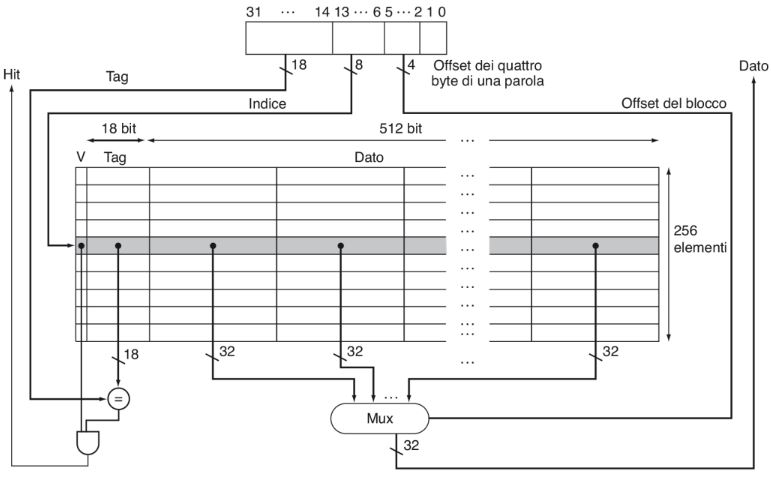
\includegraphics[width = 12cm]{Capitoli/CPU/imgCpu/hit_miss.JPG}
    \caption{HIT e MISS}
    \label{fig:hit_miss}
\end{figure}

Un accesso alla cache può causare MISS per tre motivi: 
\begin{enumerate}
    \item \textit{Cold start}: è la prima richiesta del dato/istruzione. Blocchi più grandi contengono più dati/istruzioni e il numero di cold miss diminuisce;
    \item \textit{Conflict}: il blocco è stato sovrascritto per via del grado di associatività della cache. Le cache con più vie hanno meno conflitti.
    \item \textit{Capacity}: il blocco è stato sovrascritto per via della capienza della cache. Con un maggior numero di linee si ottengono un maggior numero di richieste gestibili.
\end{enumerate}

Abbiamo visto che in fase di MISS viene creata una nuova entità nella cache, che comprende l'etichetta richiesta dal processore e una copia del dato nella memoria principale. Ma come si aggiorna la memoria principale quando il dato modificato è in cache? Si può operare principalmente in due modi: tramite il \textit{Write through} dove ad ogni modifica viene aggiornato il blocco in memoria o con il \textit{Write back} dove il blocco viene aggiornato solo quando viene sostituito.


\section{Altri tipi di mapping}
La necessità di implementare altri tipi di mapping nasce dalla richiesta di un miglioramento nelle percentuali di HIT. Infatti con il Direct Mapping ogni blocco viene salvato in una linea fissata (che dipende dal numero di blocco), questo ci premette di avere un hardware più semplice e meno costoso (è facile determinare in quale linea cercare il dato), ma allo stesso tempo, blocchi diversi sono mappati sulla stessa linea, quindi se gli accessi a quei blocchi si alternano si verificano molti miss.

Un'altro tipo di mapping è il \textit{Fully-associative mapping}, dove un blocco può essere posto in una linea qualsiasi. Questo garantisce massime prestazioni di flessibiltà ma comporta la realizzazione di un hardware più complesso e più costoso.

La migliore soluzione è implementare il \textit{Set-associative mapping}, dove le linee sono organizzate in S insiemi (set) e ogni blocco è disposto in una delle linee del set fissato.

\begin{figure}
    \centering
    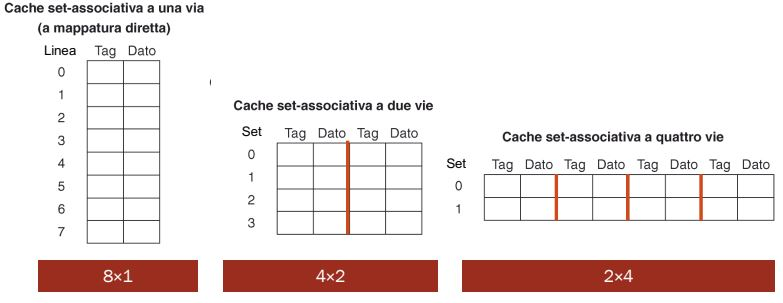
\includegraphics[width=14cm]{Capitoli/CPU/imgCpu/tipi-set-mapping.JPG}
    \caption{Tipi di set associative mapping}
    \label{fig:tipi_set_mapping}
\end{figure}

A seconda del numero di blocchi possiamo avere vari tipi di set associative mapping. In Figura \ref{fig:tipi_set_mapping} ad esempio sono mostrati tre tipi di set mapping con 8 blocchi.

Possiamo ora rappresentare un'esempio di cache set-associativa a 4 vie con blocco da 1 word, vedi Figura \ref{fig:Cache set-associativa}
\begin{figure}[ht]
    \centering
    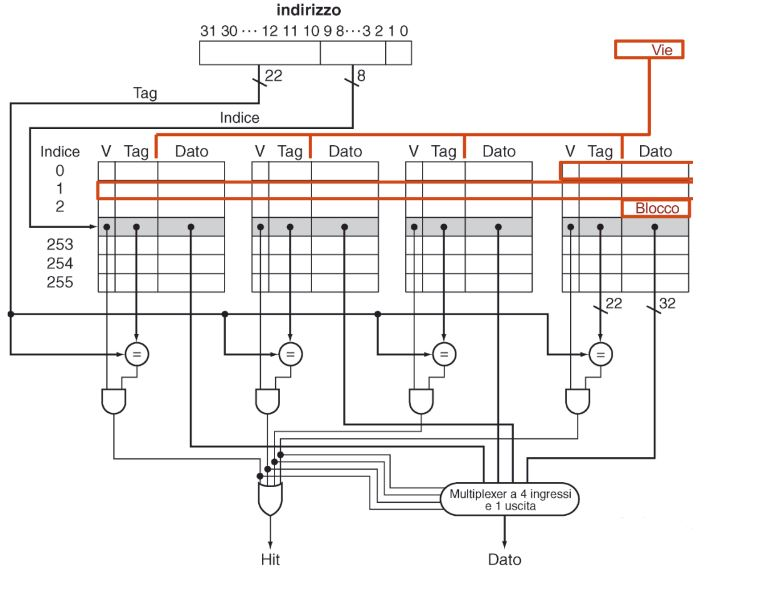
\includegraphics[width=14cm]{Capitoli/CPU/imgCpu/Cache set-associativa.JPG}
    \caption{Cache set-associativa a 4 vie con blocco da 1 word}
    \label{fig:Cache set-associativa}
\end{figure}

Per ogni via abbiamo una "tabella" che contiene S set (tanti quante sono le vie) con blocchi di N word.
Ogni linea contiene 1 bit di validità (ed eventualmente i bit \verb|Used| e \verb|Dirty|) il tag da 32 bit composto da bit di offset e bit di indice di linea e il blocco da 8 [bit] × numero di byte.

Il grande vantaggio relativo all'utilizzo di un mapping di questo tipo riguarda l'attività dei dati. Infatti, implementando più vie per linea, i dati memorizzati saranno sovrascritti con meno frequenza in quanto saranno meno le possibilità di collisioni. Viene quindi naturale chiedersi: quando un set della cache è pieno quale blocco va sostituito? Si possono utilizzare diversi approcci ad esempio si può sostituire il blocco "più vecchio" LRU (\textit{Least Recently Used}), oppure si può rimpiazzare il blocco "meno usato" LFU (\textit{Least Frequently Used}) o ancora si può cambiare con un blocco a caso (\textit{Random}).

Modificare il blocco più vecchio richiederebbe di associare un bit (\verb|Used|) a ciascuna linea e ad ogni accesso modificare \verb|Used = 1|. Il valore sarà azzerato allo scadere di un intervallo di tempo così da avere le linee con \verb|Used = 1| più recenti mentre quelle con \verb|Used = 0| più vecchie. Un'implementazione di questo tipo risolve il problema iniziale ma è sicuramente costoso mantenere questa informazione. Per sostituire il blocco meno usato, invece, si può associare un contatore a ciascun set ed aggiornarlo ad ogni accesso. Anche in questo caso però abbiamo una limitazione, ovvero l'hardware risultante sarà necessariamente più complesso.

\section{Cache multi-livello}
Una cache multi-livello è formata da n cache impilate. In questo tipo di struttura è facile vedere come ogni HIT fornisce i dati a tutti i livelli superiori, mentre le MISS fanno richieste al livello subito inferiore. 

In un sistema formato da cache multiple in parallelo, però, alcuni processi diversi potrebbero contemporaneamente accedere/modificare gli stessi dati. Per risolvere questo problema si possono collegare tra loro le cache in modo che ciascuna abbia nozione di cosa fanno le altre, e successivamente implementare la replicazione e migrazione di informazioni tra le cache.
Per progettare un controllore di cache possiamo usare un \textit{Automa a Stati Finiti (FSA)} (vedi Figura \ref{fig:FSA-cache}).

\begin{figure}
    \centering
    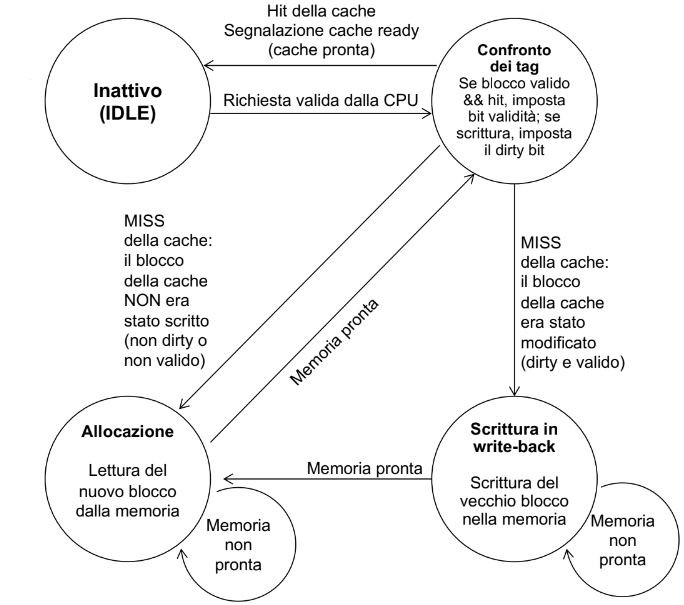
\includegraphics[width = 10cm]{Capitoli/CPU/imgCpu/FSA-cache.JPG}
    \caption{Automa a Stati Finiti della cache}
    \label{fig:FSA-cache}
\end{figure}

I 4 stati sono: attesa della richiesta (\textit{idle}); ricerca del blocco in cache (\textit{confronto dei tag}); lettura del blocco dalla memoria (\textit{allocazione}); scrittura del blocco in memoria (\textit{write-back}).

Utilizzare questo automa è un'ottimo punto di partenza, ma non risolve il problema iniziali. Infatti, più processori continuano a condividono la stessa memoria fisica (ad esempio, nei sistemi multi-core) e possono accedere contemporaneamente agli stessi dati tramite cache diverse (lo stesso blocco è presente in due copie diverse in due cache separate). Vogliamo quindi risolvere i problemi di coerenza e consistenza, dove per \textit{coerenza} si indica quale valore deve essere restituito da una lettura, mentre per \textit{consistenza} si indica quando, effettuata una scrittura, il dato sarà finalmente disponibile.

La soluzione definitiva consiste nell'implementare un \textit{protocollo di snooping}: ogni cache che contiene un blocco ne ha anche lo stato di condivisione nelle altre cache; le cache sono collegate da un bus o una rete che permette a ciascuna di sbirciare (snoop) le altre per aggiornare lo stato di condivisione del blocco; è sufficiente la trasmissione delle MISS e delle scritture da una cache a tutte le altre.



\chapter{Memoria virtuale}
In un sistema multi-processo la gestione della memoria è un argomento assai delicato. La memoria principale può non essere sufficiente per tutte le operazioni che devono essere effettuate, si vuole, in tal senso, rendere lo spazio di memoria per i processi indipendente dal limite della memoria disponibile.

Un'idea che viene utilizzata per ovviare a questo problema è: 
\begin{enumerate}
    \item produrre degli indirizzi \textit{"virtuali"} (fittizi), che vengono successivamante trasformati in indirizzi "fisici" per accedere alla vera posizione dei dati;
    \item suddividere la memoria in pagine, presenti in memoria fisica solo se necessario altrimenti memorizzate in una più lenta.
\end{enumerate}

In questo modo lo spazio di indirizzamento di un processo si semplifica e gli spazi di memoria dei processi vengono separati e protetti da accessi esterni. 

\begin{figure}[H]
    \centering
    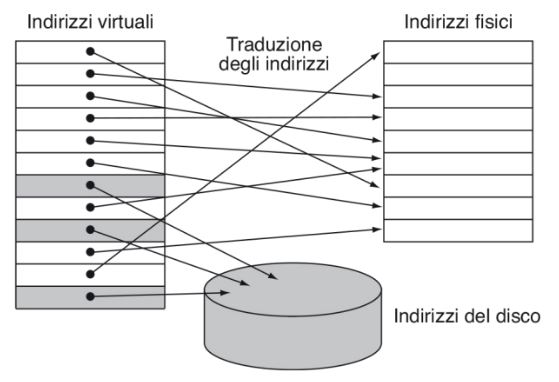
\includegraphics[width = 10cm]{Capitoli/CPU/imgCpu/memoria_virtuale.JPG}
    \caption{Memoria virtuale}
    \label{fig:memoria-virtuale}
\end{figure}

\section{Mapping degli indirizzi virtuali}
L'indirizzo virtuale viene diviso in due campi il \textit{numero di pagina} virtuale e l'\textit{offset} (esattamente come per la cache). Questi dati vengono utilizzati per costruire una tabella delle pagine (\textit{page table}), ossia una tabella contenente l'indirizzo delle pagine tramite cui si otterranno i relativi dati in memoria. 

La page table contiene tre campi per ogni processo: \verb|Valid|, \verb|Dirty| e \verb|Used| in base ai quali possiamo capire se l'indirizzo desiderato è presente o meno. In particolare se \verb|Valid| è 0 vuol dire che si sta chiedendo per la prima volta una page, quindi la tabella indica l’indirizzo in memoria di massa e viene lanciata un’eccezione di \verb|Page Fault| che richiede al sistema operativo di recuperare la pagina e inserirla in memoria fisica. In tutti gli altri casi, la tabella indica l’indirizzo in memoria principale per ottenere il dato (sono necessari almeno 2 accessi: alla page table e alla memoria principale).

\begin{figure}[H]
    \centering
    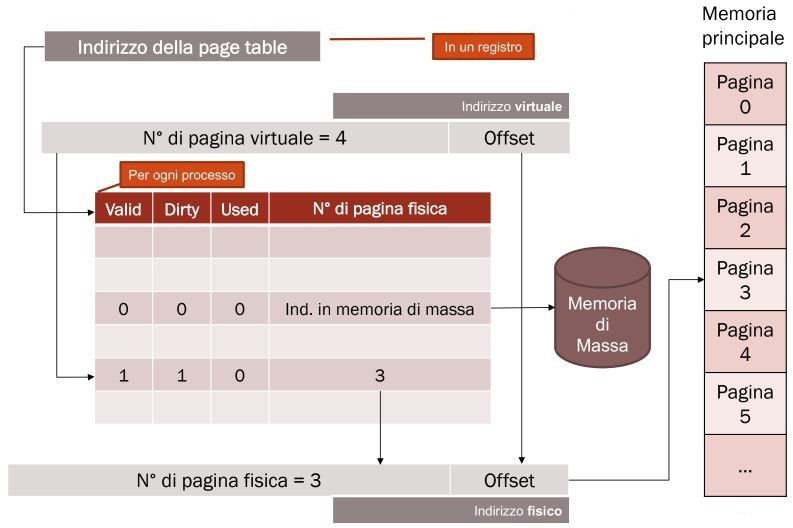
\includegraphics[width = 12cm]{Capitoli/CPU/imgCpu/page_table.JPG}
    \caption{Page table}
    \label{fig:page-table}
\end{figure}

Come per la cache occorre sostituire pagine già usate e mantenere la coerenza dei dati. Rimpiazziamo le page tramite vari approcci:
\begin{itemize}
    \item LRU (\textit{Least Recently Used}) si sostituisce la pagina utilizzata meno di recente e si imposta il bit \verb|Used| della page table a 1;
    \item LFU (\textit{Least Frequently Used}) si sostituisce la pagina utilizzata meno di frequente (richiede un contatore delle frequenze);
    \item \textit{Random} si sostituisce una pagina a caso.
\end{itemize}

e riscriviamo le page impostando il bit \verb|Dirty| della page table a 1 per indicare che la pagina è stata modificata in memoria.

Per rendere più veloce l’accesso utilizza un \textit{Table Lookaside Buffer} (TLB) che interagisce con le pagine più usate, può essere visto come una cache o meglio ancora come i preferiti del nostro browser. Gli indirizzi virtuali verranno dapprima cercati nel TLB, in caso di successo viene indicato l'indirizzo alla memoria fisica, altrimenti si passa il compito alla page table e si segue il metodo visto precedentemente (vedi Figura \ref{fig:casi-virtuale}).

\begin{figure}[H]
    \centering
    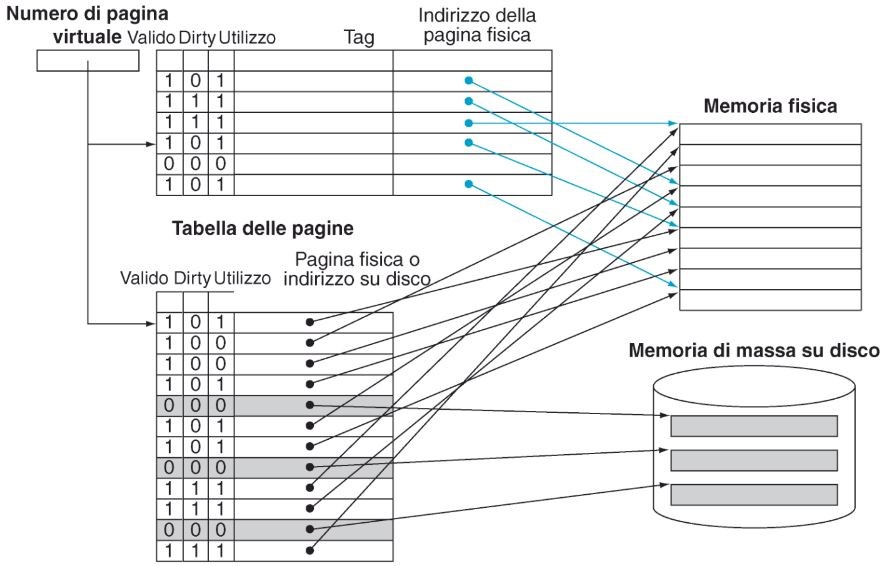
\includegraphics[width = 14cm]{Capitoli/CPU/imgCpu/tlb.JPG}
    \caption{Table Lookaside Buffer}
    \label{fig:tlb}
\end{figure}

Infine l'accesso al dato (in memoria fisica) viene effettuato dalla cache. In genere la cache sul dato può essere indicizzata dall’indirizzo fisico (va svuotata al caricamento di una nuova pagina) oppure dall’indirizzo virtuale (va svuotata durante il context switch). Di seguito sono riportati i passaggi da seguire per entrambi gli approcci:
\begin{equation*}
    \text{CPU}\xrightarrow{\text{virtuale}}\text{Cache}\xrightarrow{}\text{TLB}\xrightarrow{}\text{Page Table}\xrightarrow{\text{fisico}}\text{RAM}
\end{equation*}
\begin{equation*}
    \text{CPU}\xrightarrow{\text{virtuale}}\text{TLB}\xrightarrow{}\text{Page Table}\xrightarrow{\text{fisico}}\text{Cache}\xrightarrow{}\text{RAM}
\end{equation*}

\begin{figure}[ht]
    \centering
    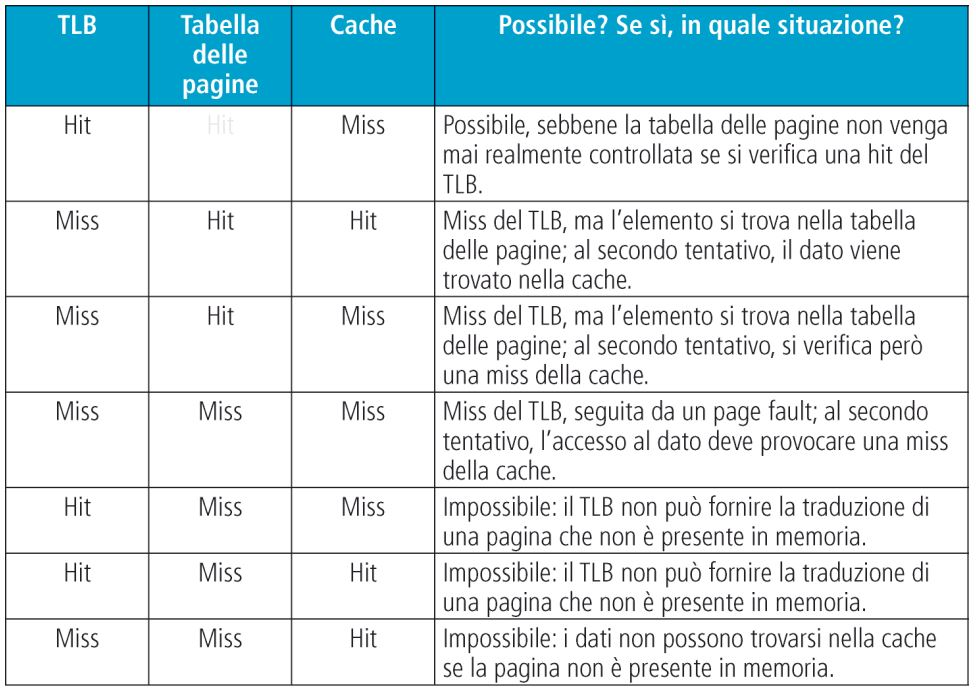
\includegraphics[width = 14cm]{Capitoli/CPU/imgCpu/casi-memoria-virtuale.JPG}
    \caption{Casistiche del mapping virtuale}
    \label{fig:casi-virtuale}
\end{figure}

\section{Supporto del Sistema Operativo}
Il sistema operativo è l'unico gestore delle pagine fisiche e risponde alle eccezioni di \verb|Page Fault| caricando in memoria fisica le pagine virtuali o modificandole sulle Page Table dei processi. In particolare:
\begin{itemize}
    \item Assegna le nuove pagine fisiche ai processi che le richiedono;
    \item Recupera le pagine dai processi che hanno terminato l’esecuzione (o che le rilasciano);
    \item Impedisce che il processo possa accedere alle pagine di altri processi;
    \item Svuota il TLB per il process switch.
\end{itemize}

La CPU, inoltre, deve impedire che il programma possa fare operazioni "pericolose" pertanto gira in 2 modi: \textit{user mode} per i programmi utente dove non sono disponibili le istruzioni per modificare Page Table e Process Table, Interruzioni ecc.; \textit{kernel mode} solo per il Sistema Operativo dove sono disponibili tutte le istruzioni.